\section{Study Design}
\label{sec:study_design}

To understand the motivations behind the creation and maintenance of variant forks we conducted an online survey with 112 maintainers of variant forks. In this section, we explain how we (i) designed the survey protocol; (ii) collected mainline--variant pairs and extracted the maintainers of the variant forks; and (iii) recruited the survey participants.

%we  and then . Next, we designed and developed a survey protocol that we used to recruit the participants.
 %The survey was run in April 2021 with the goal of understanding why developers create and maintain variant forks.

\subsection{Survey Protocol Design}
\label{sec:protocal}

%Since our aim was to learn from a large number of participants, we opted to use surveys that scales well as compared to interviews.
%\tm{I do not understand the sentence "we opted to use surveys scale well", something is incorrect in this sentence.}
Relying on the knowledge gained from literature, especially the motivations presented in Section~\ref{sec:motivations},
\cd{I would drop the first part of the section, as you already had a stronger motivation for the survey in the beginning} we designed a 12-question survey that would last at most 15 minutes.
\cd{It might help to state that you followed the best practices of our community in designing the survey, and refer to a book.}
The questions were designed so that they cover the two research questions of this paper.
%We designed the questions in such a way that the participants could choose the  reason from the provided options that best suited their motivations for forking.
8 of the 12 questions are close-ended and respondents can answer these questions either via multiple choice or Likert scales.
For these questions, the set of possible answers originated from our review of the literature.
We provided an optional free-text form for 3 of the 8 close-ended questions to give respondents the opportunity to share additional thoughts and feedback.
The 4 remaining questions are open-ended.

All questions were carefully formulated so as not to lead respondents to opt for a specific answer. We validated these questions (1) by subjecting them to the critical eye of many colleagues; and (2) by conducting informal mini-runs of the survey with a limited group of participants to obtain their feedback on it.

\ad{@John: I believe it would be nice to provide a link to the survey to that readers can see exactly what we asked. If you do so, please remember that SANER follows a double-blind review process, so the survey should be anonymized.}


\subsection{Identifying variant projects and participants}
\label{sec:forks_and_participants}

Given the scope of the survey, we aim to target respondents who are involved in the creation and maintenance of variant projects.% and possibly potentially competing.\tm{The "and possibly potentially competing" is unclear: what is possibly and potentially competing with what?}
Therefore, we first need to identify such variants.
To this end, we relied on two data sources, namely \librariesio and \gh.

\librariesio contains metadata about projects distributed through various package registries. We collected the metadata for all projects of some of the largest package registries (\textsf{npm, Go, Maven, PyPI} and \textsf{Packagist}) and we relied on this metadata to identify those projects that are variants of another one, following the variant identification method proposed by  Businge et al.~\cite{businge:emse:2021,businge:benevol:2020}. %The authors argue that, if a fork has distributed its package releases on a package registries, then one can be certain that it is a variant fork and very unlikely to be social fork.
We only considered those variants that are actively maintained in parallel to their mainline counterparts. We extracted variants for which the mainline--variant pairs are created before 2019-04-01 and updated after 2020-04-01. We wanted variants that have existed for at least one year and are not more than one old since the last commit from the time we collected the dataset, since we are interested in active projects.
%\tm{The choice of this start and end date is not motivated.}
At the end of this process, we have \textit{227 mainline–variant project pairs}.

In addition to these mainline-variant pairs distributed through package registries, we also collected pairs of projects from \gh.
We started by looking for mainline projects.
Using \gh search endpoint, we looked for \emph{popular} (i.e., $>50$ stars and forks), \emph{long-lived} (i.e., created before 2018) and \emph{active} (i.e., still updated in 2020) repositories. Since our interest is on software projects, we focused on repositories whose main language is one of the 17 most popular ones (e.g., \textsf{JavaScript, Java, Go, Python, Ruby, C}, etc.). \ad{@John: how did you select these 17 languages?}
Then, for all the mainline projects we found, we looked at their forks to identify variant forks. Collecting variant forks from \gh is subject to many threats. Previous studies have shown that the majority of forks on \gh are inactive~\cite{Businge:Android:2019,Businge:2017} or are social forks~\cite{businge:2018icsme}.
To mitigate these threats, we first filtered out forks based on a set of heuristics (e.g., $\geq 10$ stars, $\geq 10$ commits ahead of the mainline, $\geq 5$ closed pull requests, diverging \textsf{README} files, etc.).
\cd{Here I would list all heuristics used rather than use examples and remain vague.}
Then, we manually verified all the remaining forks to make sure that they correspond to variant forks of the corresponding mainline projects.
At the end of this process, we obtained \textit{264 additional mainline-variant project pairs}.
% Furthermore, since we had to manually verify the final dataset as well as reduce the number of false positives, we came up with restrictive magic numbers to achieve our goal.
% We searched mainline repositories written in the 17 popular programming languages on \gh that include: \textsf{JavaScript}, \textsf{Java}, \textsf{Go}, \textsf{Python}, \textsf{Ruby}, \textsf{C}, having $>50$ forks and and also having a long development history (created before 2018-04-01 and updated after 2020-04-01).
% For each mainline, we extracted forks that were created before 2019-04-01 and updated after 2020-04-01, having $\geq 10$ stargazers, having $\geq 10$ commits ahead of the mainline (unique commits), having $\geq 5$ closed pull requests, and where the fork and mainline differ in the contents of the \textsf{readme.md} file for description.
% We manually verified that the mainline and fork indeed belonged to two different projects by reading and comparing the contents of their \textsf{readme.md}. Using this process, \textit{we obtained an additional 225 mainline–variant project pairs}.

%The mainline-variant project pairs we obtained so far correspond to \emph{attached forks}, in the sense that a direct traceability link exists between the mainline repository and the variant fork (i.e., the variant repository is \emph{officially} a \emph{fork of} the mainline repository on \gh).
%In contrast, \emph{detached forks} correspond to those repositories that were ``manually'' cloned from the mainline's one with no technically explicit traceability link.
%In the following, we will distinguish between two kind of variant projects, corresponding to \emph{attached forks} and \emph{detached forks}.
%\emph{Attached forks} correspond to those projects that are still \emph{attached} to the mainline in the sense that a direct traceability link exists between the mainline and fork (e.g., the \emph{fork of} attribute in \gh). On the other hand, \emph{detached forks} are those forks that were ``manually'' cloned and, consequently, whose repository does not maintain a link with the mainline.
%\ad{@John: Here we need to have some words to explain why you wanted to have \emph{detached forks} as well. It might be good to add an example of such a \emph{detached fork}.}

%To identify such detached forks, we relied again on \gh search endpoint. We searched for repositories that are not labelled as ``forks'' by \gh but that do contain ``\emph{fork of}'' in their description. We filtered out the resulting repositories the same way we did before with attached forks. We then manually inspected these repositories and manually identified the mainline projects they are variant of.
%\nd \textit{Identifying detached variant projects}. We used \gh search feature looking for repositories that are not referred as ``forks'' but that do contain ``fork of'' in their description and both the mainline and variant projects are actively maintained (i.e., were forked before \texttt{2019-04-01} and updated after \texttt{2020-04-01}; the mainline and variant have at least 100 commits after the fork date). We also manually verified that indeed the mainline and variant are indeed different projects being maintained in parallel by reading their \texttt{readme.md} pages. Using this process,
%This lead us with \textit{40 additional mainline–variant project pairs}.

Overall from the three methods we followed, we collected \textbf{a total of 491 mainline--variant pairs}.
%\ad{@John: 225 + 227 + 40 = 492.}



\subsection{Participant Recruitment}

Based on this list of 491 mainline-variant pairs, we identified contributors that had integrated at least one pull request into the variant (i.e., contributors that are maintainers of the project).
We retrieved their public-facing emails (if available) using \gh API, carefully following the \gh Privacy Statement while doing so.\footnote{https://docs.github.com/en/github/site-policy/github-privacy-statement}

At end of this process, we could contact a total of 762 variant maintainers from the 491 variant projects, and managed to attract \textbf{a total of 112 respondents (response rate of 15\%) representing a total of 105 variant fork repositories (response rate of 21\%)}.
All participants were asked to read and accept an informed consent form before taking part in the survey.

%When distributing the survey protocol, we customized each of the \textit{email message content} using the respondents personal information. For example the email title was customized as follows\footnote{Academic Research on motivation of creating forks - \texttt{[fork\_name]}}. The body of the email message was also customized as follows\footnote{[\ldots] we have identified your \gh repository \texttt{[fork\_name]} as a variant fork of the mainline \texttt{[mainline\_name]}}.

\begin{figure}[ht]
\begin{center}
    \centering
    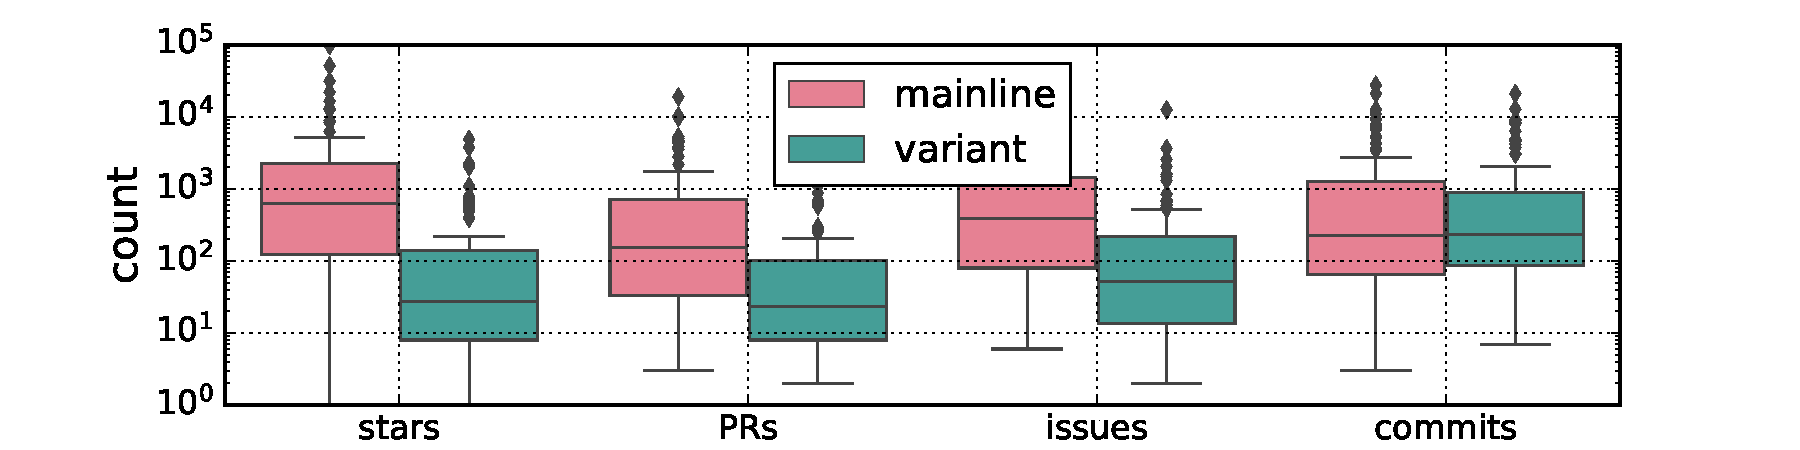
\includegraphics[width=\columnwidth]{pdfs/stats.pdf}
    \caption{Distribution of selected metrics. PRs, issues and commits are counted after the fork date for both mainline and variant.}
    \label{fig:stats}
\end{center}
\vspace{-.3cm}
\end{figure}

Fig.~\ref{fig:stats} shows the distributions of stars, pull requests, issues and commits for the mainline-variant pairs we selected. Only the 105 projects for which at least one maintainer took part in the survey were considered.

\ad{@John: I could not rewrite the next paragraph because I do not really understand it (and its purpose). I guess we need at least one or two sentences to explain the goal of the figure, and what can be observed from it.}
Apart from the stars where we consider all in the mainline\cd{For me this subsentence was the only part I did not understand.}
, we count all (closed + open) PRs, issues, and commits (only main branch) after the fork date. While it is not surprising that the counts for mainline metrics are always higher than those of the variants, it is interesting that most variants are also popular in stars, pull requests and issues counts. This gives us confidence that we are studying real variants as opposed to social forks.
%\ad{I propose to move Fig.~\ref{fig:stats} and the corresponding text to previous section.}


\subsection{Analysis}
\label{sec:card_sorting}

\ad{@John: I'm not really used to card sorting, but I couldn't really understand the whole process you followed after having read the following paragraph. Please add some sentences to explain why card sorting is needed and which ``issue(s)'' it solves.}

We used card sorting~\cite{zimmermann2016card}, on the 3 open-ended questions which provides a framework to ascertain the meaning and summarize overarching themes of responses within the context of the research question. In the analysis, we grouped similar responses to the open-ended questions into codes. We did not start with any pre-defined codes in mind, but instead derived the codes from the data, iterating as many times as needed until reaching a saturation point. The first iteration of coding was performed by the first author of the paper, and any responses the first author was unsure of were decided by discussion with another\cd{the second?} author. Once the first two authors agreed on the codes, a virtual meeting was agreed upon where all the other authors joined and discussed the resulting codes and themes and through negotiated agreement~\cite{Garrison:2006}. This approach allowed us to remove duplicates and, in some cases, to generalize or specialize themes, which we will discuss in the later sections of this paper.
